% !TEX root = main.tex

\section{Data samples and event selection}
\label{sec:Selection}

%Throughout the note, we abbreviate $\Bs\to\Ds X_{s}(\to\kaon\pion\pion)$ and $\Bs\to\Ds X_{d}(\to\pion\pion\pion)$. 
%, identifying $X_{s}\to\kaon\pion\pion$ and $X_{d}\to\pion\pion\pion$ as the various resonances through which the decays proceed. 

\subsection{Stripping and Trigger selection}

The dataset used for this analysis corresponds to $1 \invfb$ of proton-proton collision data
collected in 2011 with a centre of mass energy $\sqrt{s} = 7\tev$,  $2 \invfb$  collected in
2012 with $\sqrt{s} = 7\tev$ and $2 \invfb$  collected in
2015/2016 with $\sqrt{s} = 13\tev$.
Candidate $\Bs\to\Ds\kaon\pion\pion$ ($\Bs\to\Ds\pion\pion\pion$) decays are reconstructed using the
\textsf{B02DKPiPiD2HHHPIDBeauty2CharmLine} (\textsf{B02DPiPiPiD2HHHPIDBeauty2CharmLine})
line of the \textsf{BHadronCompleteEvent} stream of  
\textsf{Stripping21r1} (2011), \textsf{Stripping21} (2012),
\textsf{Stripping24r1} (2015)  and \textsf{Stripping28r1p1} (2016).
%and \textsf{Stripping29r2} (2017)
Both stripping lines employ the same selection cuts, listed in Appendix \ref{sec:StripAndTrigger}, except for the PID requirement on the bachelor kaon/pion.

Events that pass the stripping selection are further required to fulfill the following trigger requirements:
at the hardware stage, the $\Bs$ candidates are required to be TOS on the \textsf{L0Hadron} trigger or TIS on \textsf{L0Global};
at Hlt1, $\Bs$ candidates are required to be TOS on the \textsf{Hlt1TrackAllL0} (\textsf{Hlt1TrackMVA} or \textsf{Hlt1TwoTrackMVA}) trigger line for Run-I (Run-II) data;
at Hlt2, candidates have to be TOS on either one of the 2, 3 or 4-body topological trigger lines or the inclusive $\phi$ trigger. 
More details on the used HLT lines are given in Appendix \ref{sec:StripAndTrigger}.

Due to a residual kinematic dependence on whether the event is triggered by \textsf{L0Hadron} or not and on the data taking condition,
the analysis is performed in four disjoint categories: 
$[\text{Run-I,}\textsf{L0-TOS}]$, $[\text{Run-I,}\textsf{L0-TIS}]$, $ [\text{Run-II,}\textsf{L0-TOS}]$ and $ [\text{Run-II,}\textsf{L0-TIS}]$,
where for simplicity we denote $\textsf{L0-TOS}$ as $\textsf{L0Hadron-TOS}$ and $\textsf{L0-TIS} $ as $ (\textsf{L0Global-TIS} \text{ and not } \textsf{L0Hadron-TOS}$).
 


\subsection{Offline selection}

The offline selection, in particular the requirements on the $D_s$ hadron, are guided by the previous analyses of 
$B_s \to D_s K/\pi$, $B_d \to D^0 \pi$ as well as the branching fraction measurement of $\Bs\to\Ds\kaon\pion\pion$ decays.
%A two-fold approach is used to isolate the signal candidates from data passing the stripping line. 
%First, loose cuts are applied to suppress the combinatorial background, 
%Following this, a multivariate classifier is trained which combines the information of several input variables, including their correlation, into one powerful discriminator
%between signal and combinatorial background. 

In order to clean up the sample and to align the Run-I to the slightly tighter Run-2 stripping selection, we apply the following loose cuts to the b-hadron:
\begin{itemize}
\item DIRA $>$ 0.99994
\item min IP $\chi^{2}$ $<$ 20 to any PV,
\item FD $\chi^{2}$ $>$ 100 to any PV,
\item Vertex $\chi^{2}$/nDoF $<$ 8.
%\item ($Z_{\Ds}-Z_{\Bs}$) $>$ 0 , where $Z_{M}$ is the z-component of the position $\vec{x}$ of the decay vertex for the $\Bs$/$\Ds$ meson.
\end{itemize}    
We reconstruct the $\Bs\to\Ds h\pion\pion$ decay through two different final states of the $\Ds$ meson, $\Ds\to\kaon\kaon\pion$ and $\Ds\to\pion\pion\pion$.
Of those, $\Ds\to\kaon\kaon\pion$ is the most prominent one,
while $\mathcal{BR}(\Ds\to\pion\pion\pion) \approx 0.2\cdot\mathcal{BR}(\Ds\to\kaon\kaon\pion)$ holds for the other. 
For the $\kaon\kaon\pion$  final state we make use of the well known resonance structure;
the decay proceeds either via the narrow $\phiz$ resonance, the broader $\Kstarz$ resonance or (predominantly) non-resonant.
Within the $\phiz$ resonance region the sample is already sufficiently clean after the stripping so that we do not impose additional criteria on the $D_s$ daughters.
For the $\Kstarz$ and non-resonant regions consecutively tighter requirements on the particle identification and the $D_s$ flight-distance are applied. 
We apply global requirements for the $\Ds\to\pion\pion\pion$ final state.



%Depending on the decay process being resonant or not, we apply additional PID requirements on this final state:
%
%\begin{itemize}
%\item resonant case: 
%\begin{itemize}
%\item $\Dsp\to\phiz\pip$, with $|M(\Kp\Km) - m_{\phiz}|$ $<$ 20 $\mevcc$ : no additional requirements, since $\phiz$ is narrow and almost pure $\Kp\Km$. 
%\item $\Dsp\to\Kstarzb\Kp$, with  $|M(\Km\pip) -m_{\Kstarz}|$ $<$ 75 $\mevcc$ :  $\dllkpi$ $>$ 0 for kaons, since this resonance is more than ten times broader than $\phiz$. 
%\end{itemize}
%\item non resonant case: $\dllkpi$ $>$ 5 for kaons, since the non resonant category has significant charmless contributions.
%\end{itemize}
%
%\begin{itemize}
%\item $\dllkpi$ $<$ 10 for all pions.
%\item $\dllppi$ $<$ 10 for all pions.
%\end{itemize}
 
 
\subsubsection{Physics background vetoes}

We veto various physical backgrounds, which have either the same final state as our signal decay, or can contribute via a single misidentification of $\kaon\to\pion$ or $\kaon\to\proton$. 
In the following, the vetoes are ordered by the reconstructed $\Ds$ final state they apply to: 

\begin{enumerate}

%\item All:
%\begin{enumerate}
%%\item $\Bs\to\Dsp\Dsm$ : $|M(\kaon\pion\pion) - m_{\Ds}| >$ 20 $\mevcc$.
%\item $\Bs\to\Ds^{-}\Kp\Km\pip$ : possible with single missID of $\Km\rightarrow\pim$, rejected by requiring $\pim$ to fulfill $\dllkpi$ $<$ 5. 
%\end{enumerate}

\item $\Ds^-\to\kaon^+\kaon^-\pion^-$

\begin{enumerate}
	\item $\Dm \to\Kp\pim\pim$: 
	possible with single missID of $\pim\rightarrow\Km$, vetoed by requiring 
	$m(\Kp K^-_\pi \pim) \ne m(D^-) \pm 30$ MeV 
	or the $\Km$ has to fulfill more stringent PID criteria depending on the resonant region.
	
	\item $\Lambda_c^- \to \Kp \bar p \pim $: 
	possible with single missID of $\bar p \rightarrow\Km$, vetoed by requiring
	$m(\Kp K^-_p \pim) \ne m(\Lambda_c) \pm 30$ MeV
	or the $\Km$ has to fulfill more stringent PID criteria depending on the resonant region.
	
	\item $\Dz\to\kaon\kaon$: $\Dz$ combined with a random $\pion$ can fake a $\Ds\to\kaon\kaon\pion$ decay, vetoed by requiring $m(\kaon\kaon) < 1840 \mev$. 
\end{enumerate}

\item $\Ds^-\to\pion^+\pion^-\pion^-$

\begin{enumerate}
        \item $\Dm \to\Kp\pim\pim$: 
%	possible with single missID of $\Km\rightarrow\pim$: $m(\pip_K \pim \pim) is shifted to lower masses and 
	
	\item $\Dz\to\pion\pion$: 
		combined with a random $\pion$ can fake a $\Ds\to\pion\pion\pion$ decay, 
		vetoed by requiring both possible combinations to have $m(\pion\pion) < 1700 \mev$.
\end{enumerate}

\item $\Ds^- \to K^- \pion^+\pion^-$

\begin{enumerate}
	\item $\Dm \to\pim \pip \pim$:  	$m(K^-_\pi \pip \pim) \ne m(D^-) \pm 30$ MeV 


	\item $\Lambda_c^- \to \Kp \bar p \pim $: 

	\item $\Dz\to\kaon\pion$: 
		combined with a random $\pion$ can fake a $\Ds\to\kaon\pion\pion$ decay, 
		vetoed by requiring both possible combinations to have $m(\kaon\pion) < 1700 \mev$.
\end{enumerate}

\end{enumerate}



\begin{enumerate}

\item $X_s \to \Kp \pip \pim$:
\begin{enumerate}
\item $\Bs\to\Ds\pion\pion\pion$
\item $\Bs\to\Dsm\Dsp$ 
\item $\Bs \to \Dsm \mu \nu X$
%: $|M(\kaon\pion\pion) - m_{\Ds}| >$ 20 $\mevcc$.
%\item $\Bs\to\Ds^{-}\Kp\Km\pip$ : possible with single missID of $\Km\rightarrow\pim$, rejected by requiring $\pim$ to fulfill $\dllkpi$ $<$ 5. 
\end{enumerate}

\item $X_d \to \pip \pip \pim$:
\begin{enumerate}
\item $\Bs\to\Ds\kaon\pion\pion$
\item $\Bs \to \Dsm \mu \nu X$
%\item $\Bs\to\Dsp\Dsm$ 
%: $|M(\kaon\pion\pion) - m_{\Ds}| >$ 20 $\mevcc$.
%\item $\Bs\to\Ds^{-}\Kp\Km\pip$ : possible with single missID of $\Km\rightarrow\pim$, rejected by requiring $\pim$ to fulfill $\dllkpi$ $<$ 5. 
\end{enumerate}

\end{enumerate}


Given the high number of $pp$ interactions per bunch crossing, a large fraction
of events have more than one reconstructed PV. 
We choose the 'best' PV to be the one to which the 
$B_s$ candidate has the smallest $\chi^2_{IP}$.
In instances where the association of the $B_s$ candidate to the best PV is wrong,
the decay time of this candidate will be incorrect. 
These wrongly associated candidates
are rejected by requiring that the $B_s$ $\chi^2_{IP}$ with respect to any other PV is sufficiently higher than with respect to the best PV 
($\Delta \chi^2_{IP} = \chi^2_{\text{IP,SECONDBEST}} - \chi^2_{\text{IP,BEST}} > 20$ ).
Events with only a single PV are not affected.

 \subsubsection{Phase space region}

Due to the comparable low masses of the final state particles  with respect to the $B_s$ mass,
there is, in contrast to for example b-hadron to charmonia or charm decays, a huge phase-space available for the $\Bs\to\Ds\kaon\pion\pion$ decay.
For the invariant mass of the $K\pi\pi$ subsystem it extends up to $3.4 \gev$.
It has however been observed that the decay proceeds predominantly through the low lying axial vector states $K(1270)$ and $K(1400)$, while
the combinatorial background is concentrated at high $K\pi\pi$ invariant masses ($m(K\pi\pi) > 2000 \mev$).
Moreover, the strange hadron spectrum above $2\gev$ is poorly understood experimentally such that an reliable extraction of the strong phase motion in that region is not possible.
We consequently choose the considered phase space region to be $m(K\pi\pi) < 1950 \mev$, which is right below the charm-strange threshold ($\Bs\to\Dsp\Dsm$).


\clearpage
\subsubsection{Training of multivariate classifier}

We use TMVA \cite{Hocker:2007ht} to train a multivariate discriminator, which is used to further improve the signal to background ratio. 
The following variables are used for the training:

\begin{itemize} 

\item max(ghostProb) over all tracks

\item cone($\pt$) asymmetry of every track, 
which is defined to be the difference between the $\pt$ of the $\pi$/$\kaon$ and the sum of all other $\pt$ in a cone of radius $r = \sqrt{(\Delta\Phi)^{2} + (\Delta\eta)^{2}}$ $<$ 1 rad around the signal $\pi$/$\kaon$ track.

\item min(IP$\chi^{2}$) over the $X_{s}$ daughters

\item max(DOCA) over all pairs of $X_{s}$ daughters

\item min(IP$\chi^{2}$) over the $\Ds$ daughters

\item $\Ds$ and $\Bs$ DIRA

\item $\Ds$ FD significance

\item max($\cos(\Ds h_{i})$), where $\cos(\Ds h_{i})$ is the cosine of the angle between the $\Ds$ and another track i in the plane transverse to the beam

\item $\Bs$ IP$\chi^{2}$, FD$\chi^{2}$ and Vertex $\chi^{2}$

\end{itemize}

Various classifiers were investigated in order to select the best performing discriminator. Consequently, a boosted decision tree with gradient boost (BDTG) is chosen as nominal classifier. 
We use truth-matched MC as signal input. 
Simulated signal candidates are required to pass the same trigger, stripping and preselection requirements, that were used to select the data samples.  
For the background we use events from the high mass sideband ($m_{\Bs candidate}$ $>$ 5600 $\mevcc$) of our data samples. 
%As shown in Fig. \ref{fig:massforBDT}, this mass region is sufficiently far away from signal structures and is expected to be dominantly composed of combinatorial background.
%For completeness, the mass distribution of preselected $\Ds\to\hadron\hadron\hadron$ candidates (where $\hadron = \pion$ or $\hadron = \kaon$) is also shown in Fig. \ref{fig:massforBDT}.    \newline
%\begin{figure}[h]
%%\vspace*{-0.4cm}
%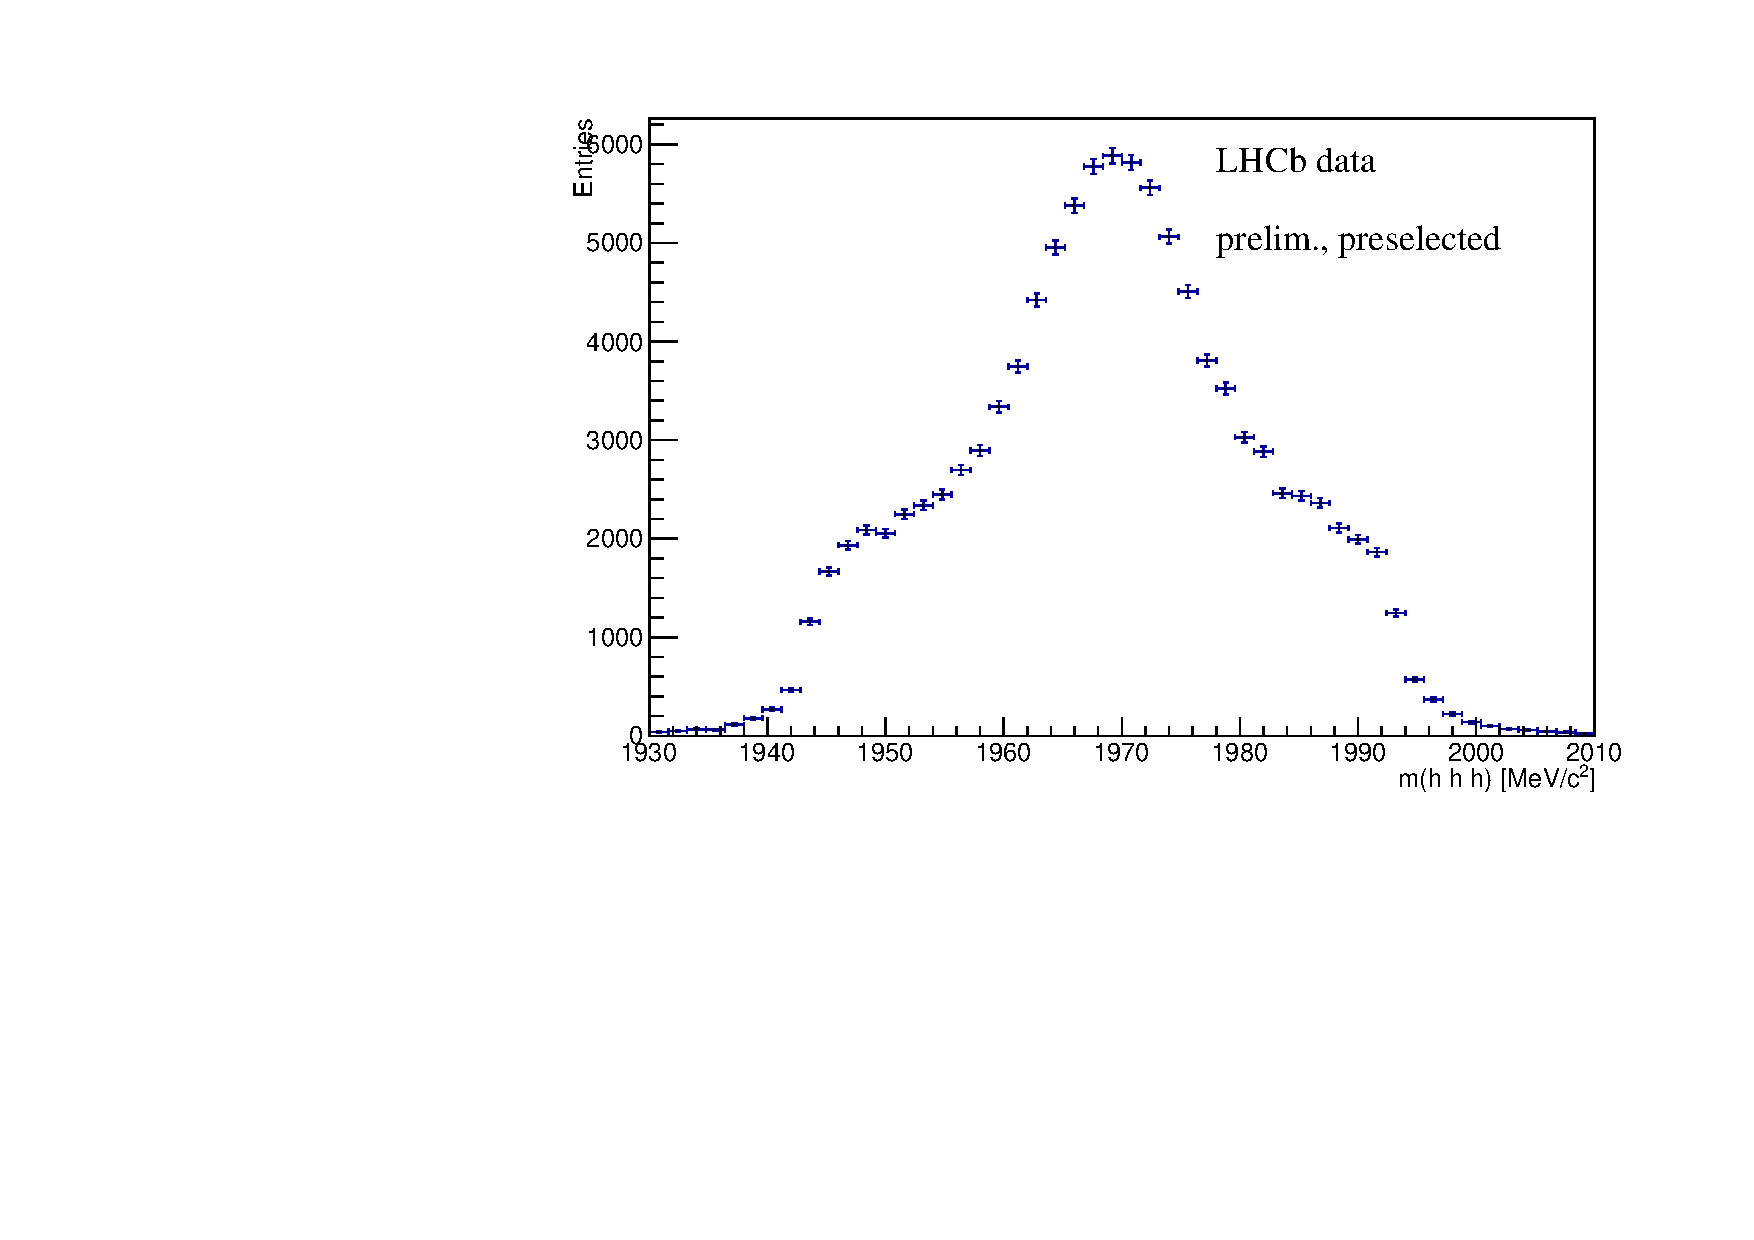
\includegraphics[height=7.0cm,width=0.49\textwidth]{figs/Ds_MM_afterpresel.pdf}
%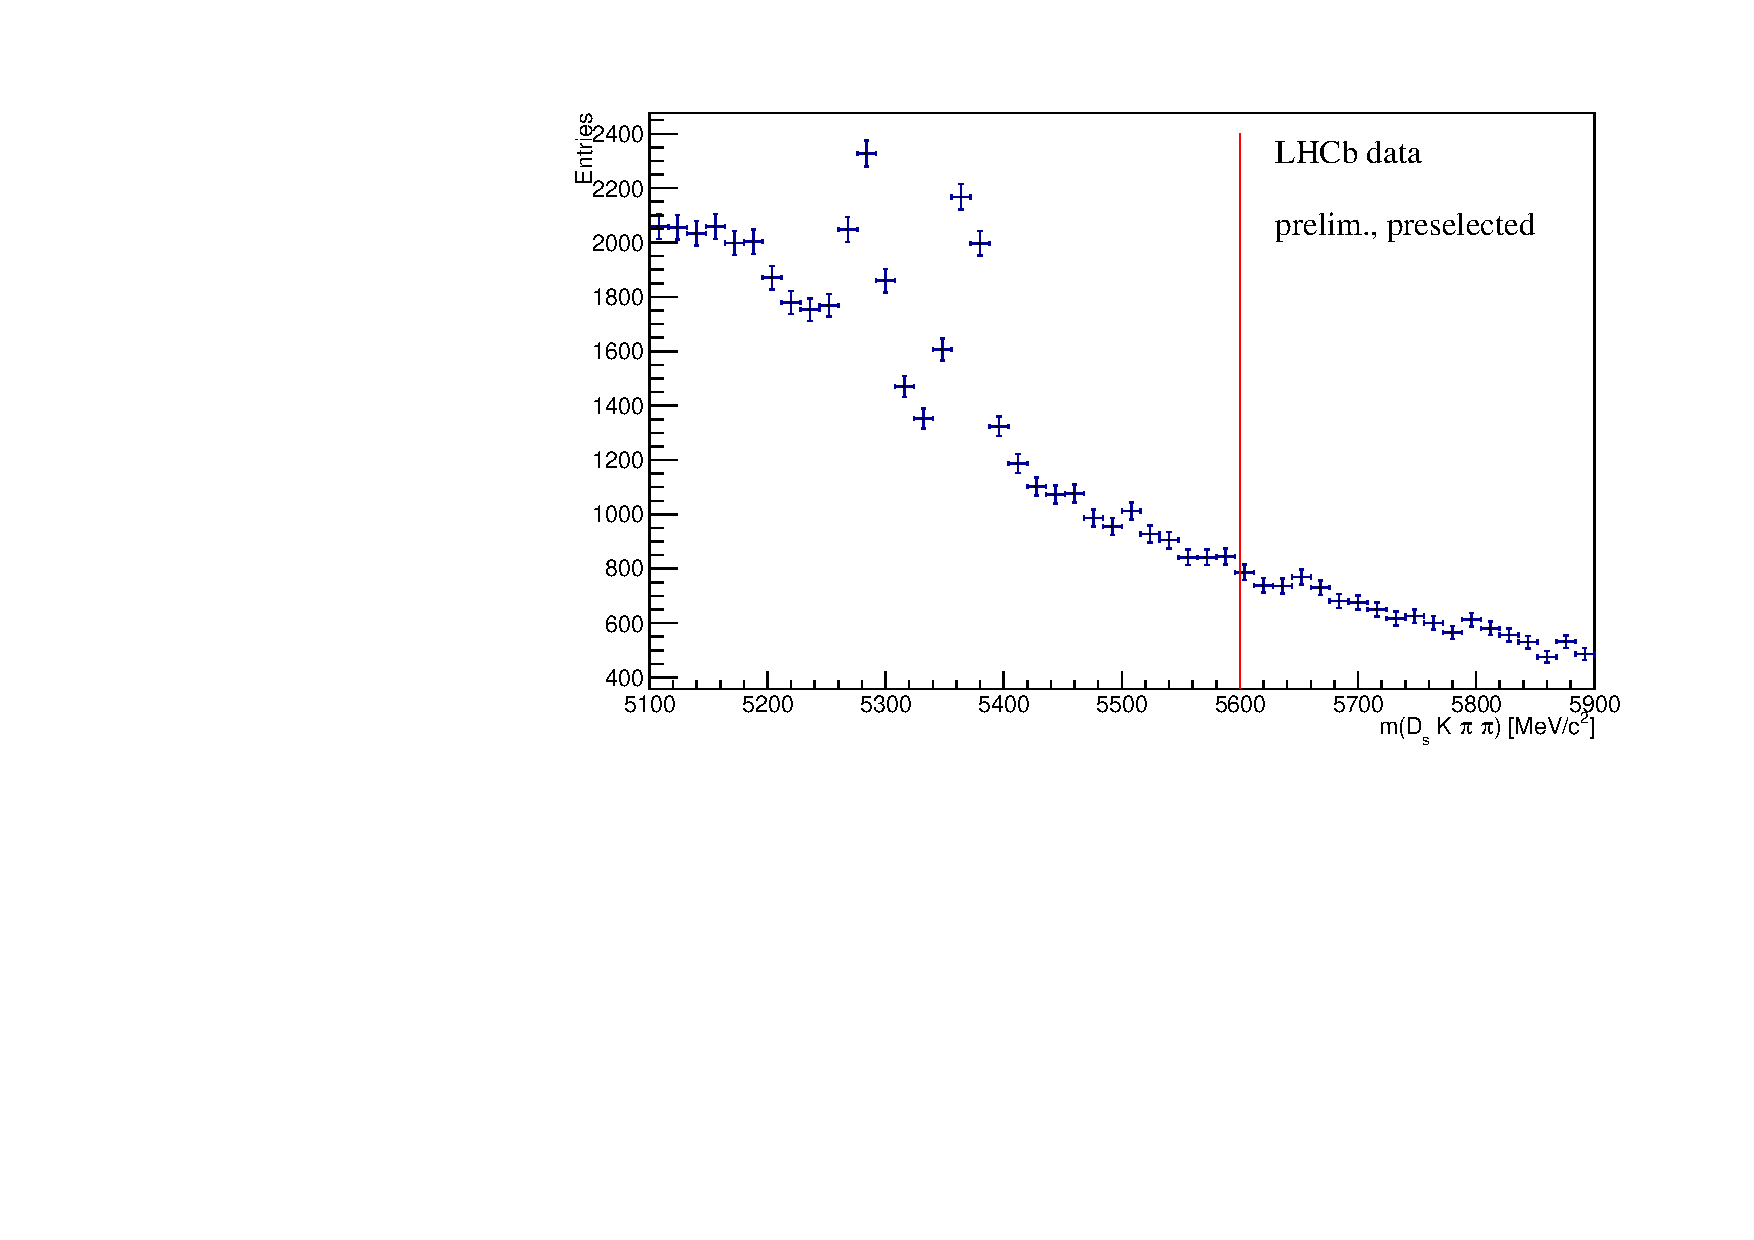
\includegraphics[height=7.0cm,width=0.49\textwidth]{figs/Bs_MM_afterpresel.pdf}
%%\vspace*{-0.2cm}
%\caption{Invariant mass distribution of preselected (left) $\Ds\to\hadron\hadron\hadron$ and (right) $\Bs\to\Ds\kaon\pion\pion$ candidates. 
%For the  $\Bs\to\Ds\kaon\pion\pion$ candidates, the region right from the red colored line with $m_{\Bs candidate}$ $>$ 5600 $\mevcc$ is used as background input for the boosted decision tree.}
%\label{fig:massforBDT}
%\end{figure}

The distributions of the input variables for signal and background and 
the BDTG output distribution are shown in the appendix.

\begin{figure}[h]
\centering
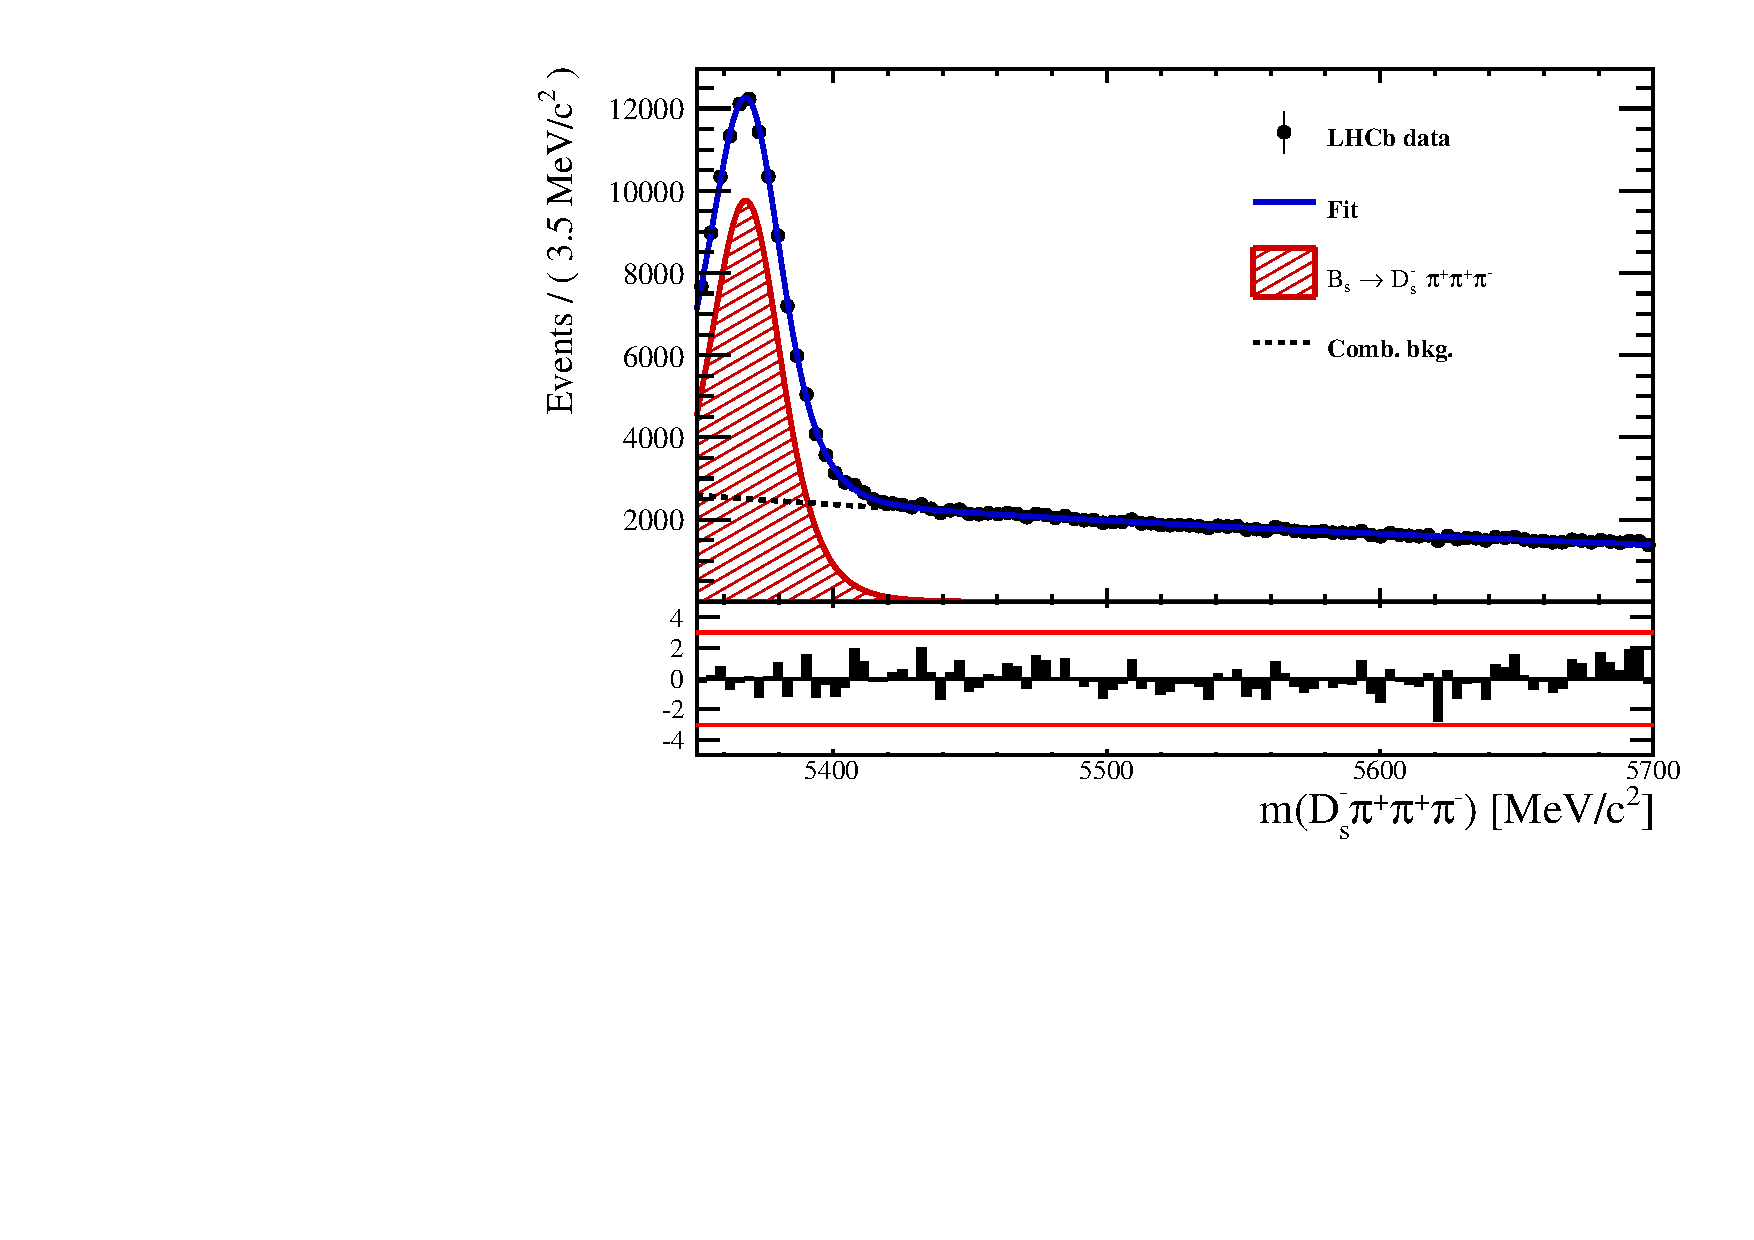
\includegraphics[height=!,width=0.45\textwidth]{figs/MassFit/norm_preselected_pull.pdf}
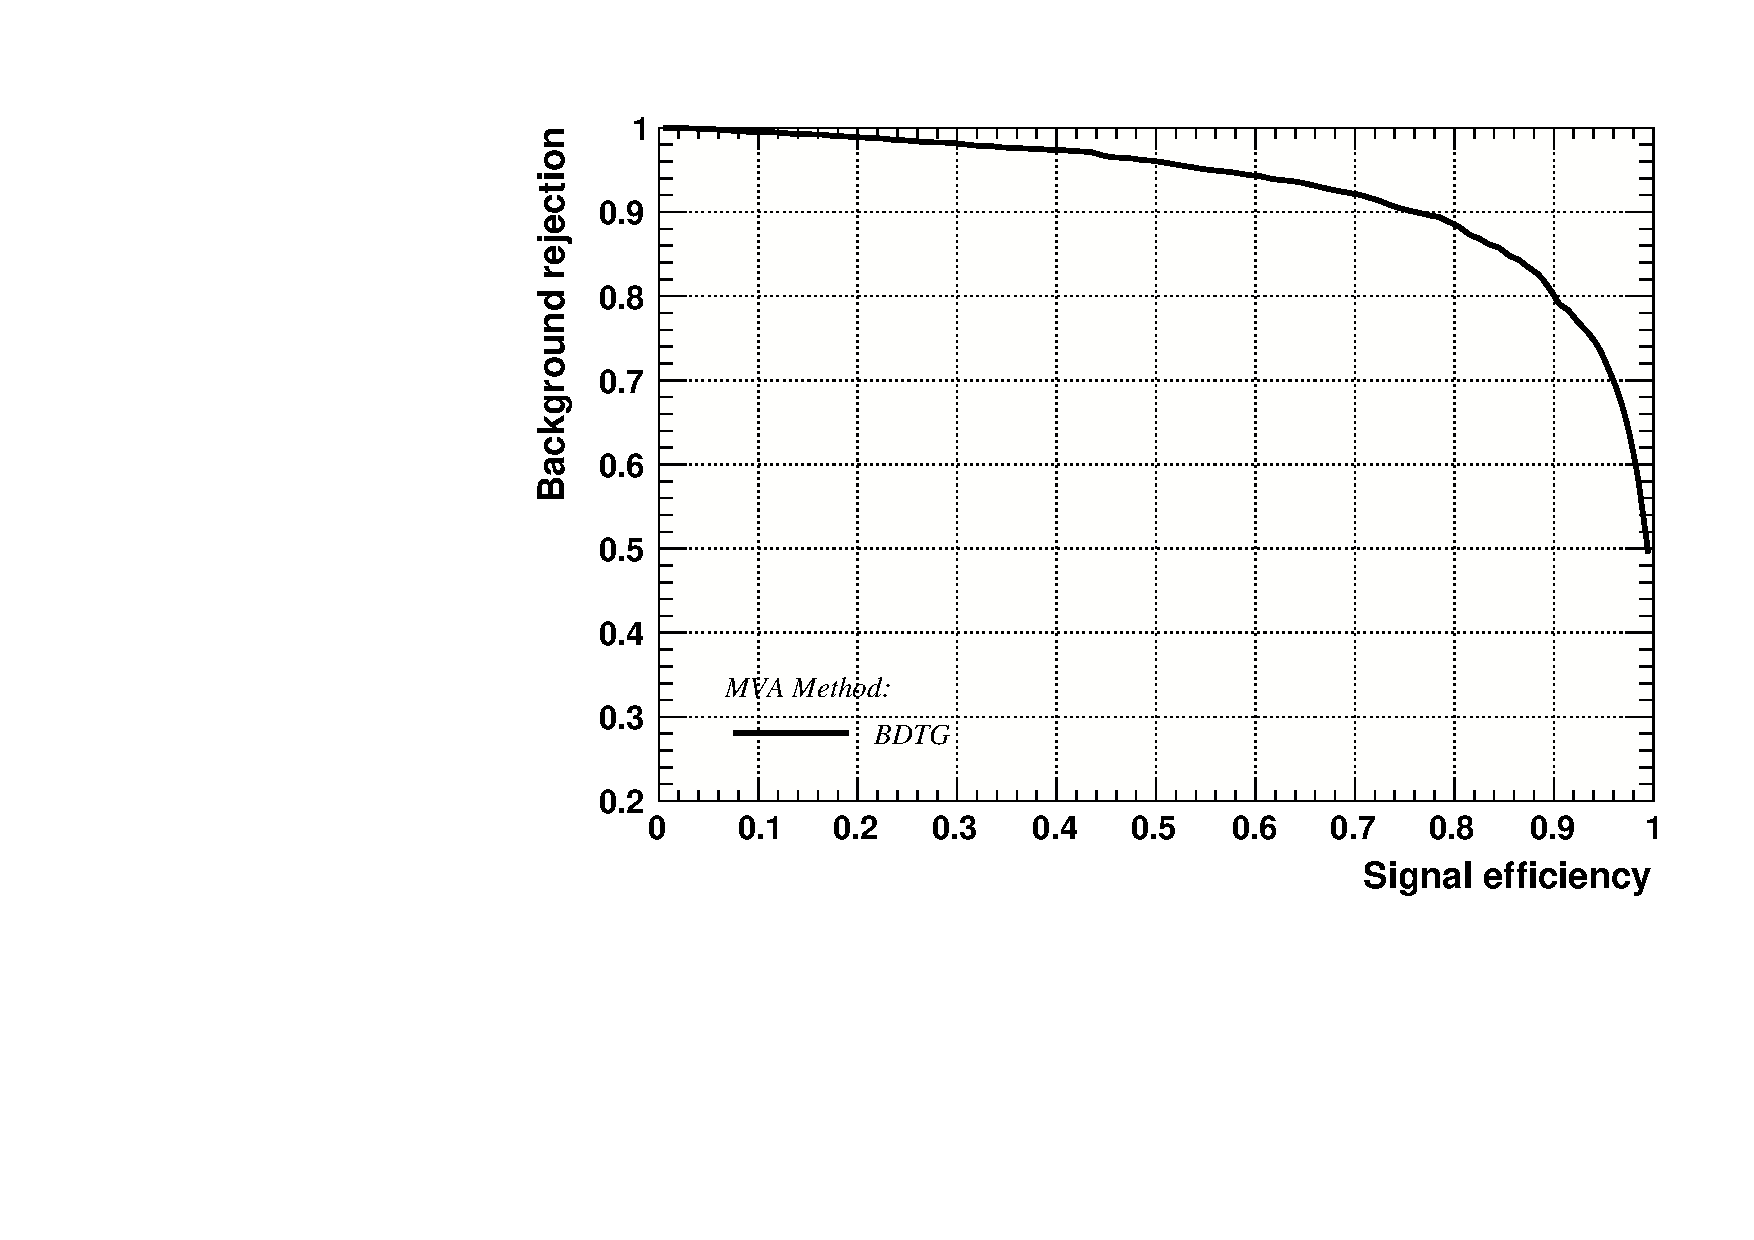
\includegraphics[height=!,width=0.45\textwidth]{figs/TMVA/BDTG_Data_run1_t0_even/rejBvsS.pdf}
\caption{}
\label{fig:}
\end{figure}


\subsubsection{Final selection}


%\begin{figure}[h]
%%\vspace*{-0.4cm}
%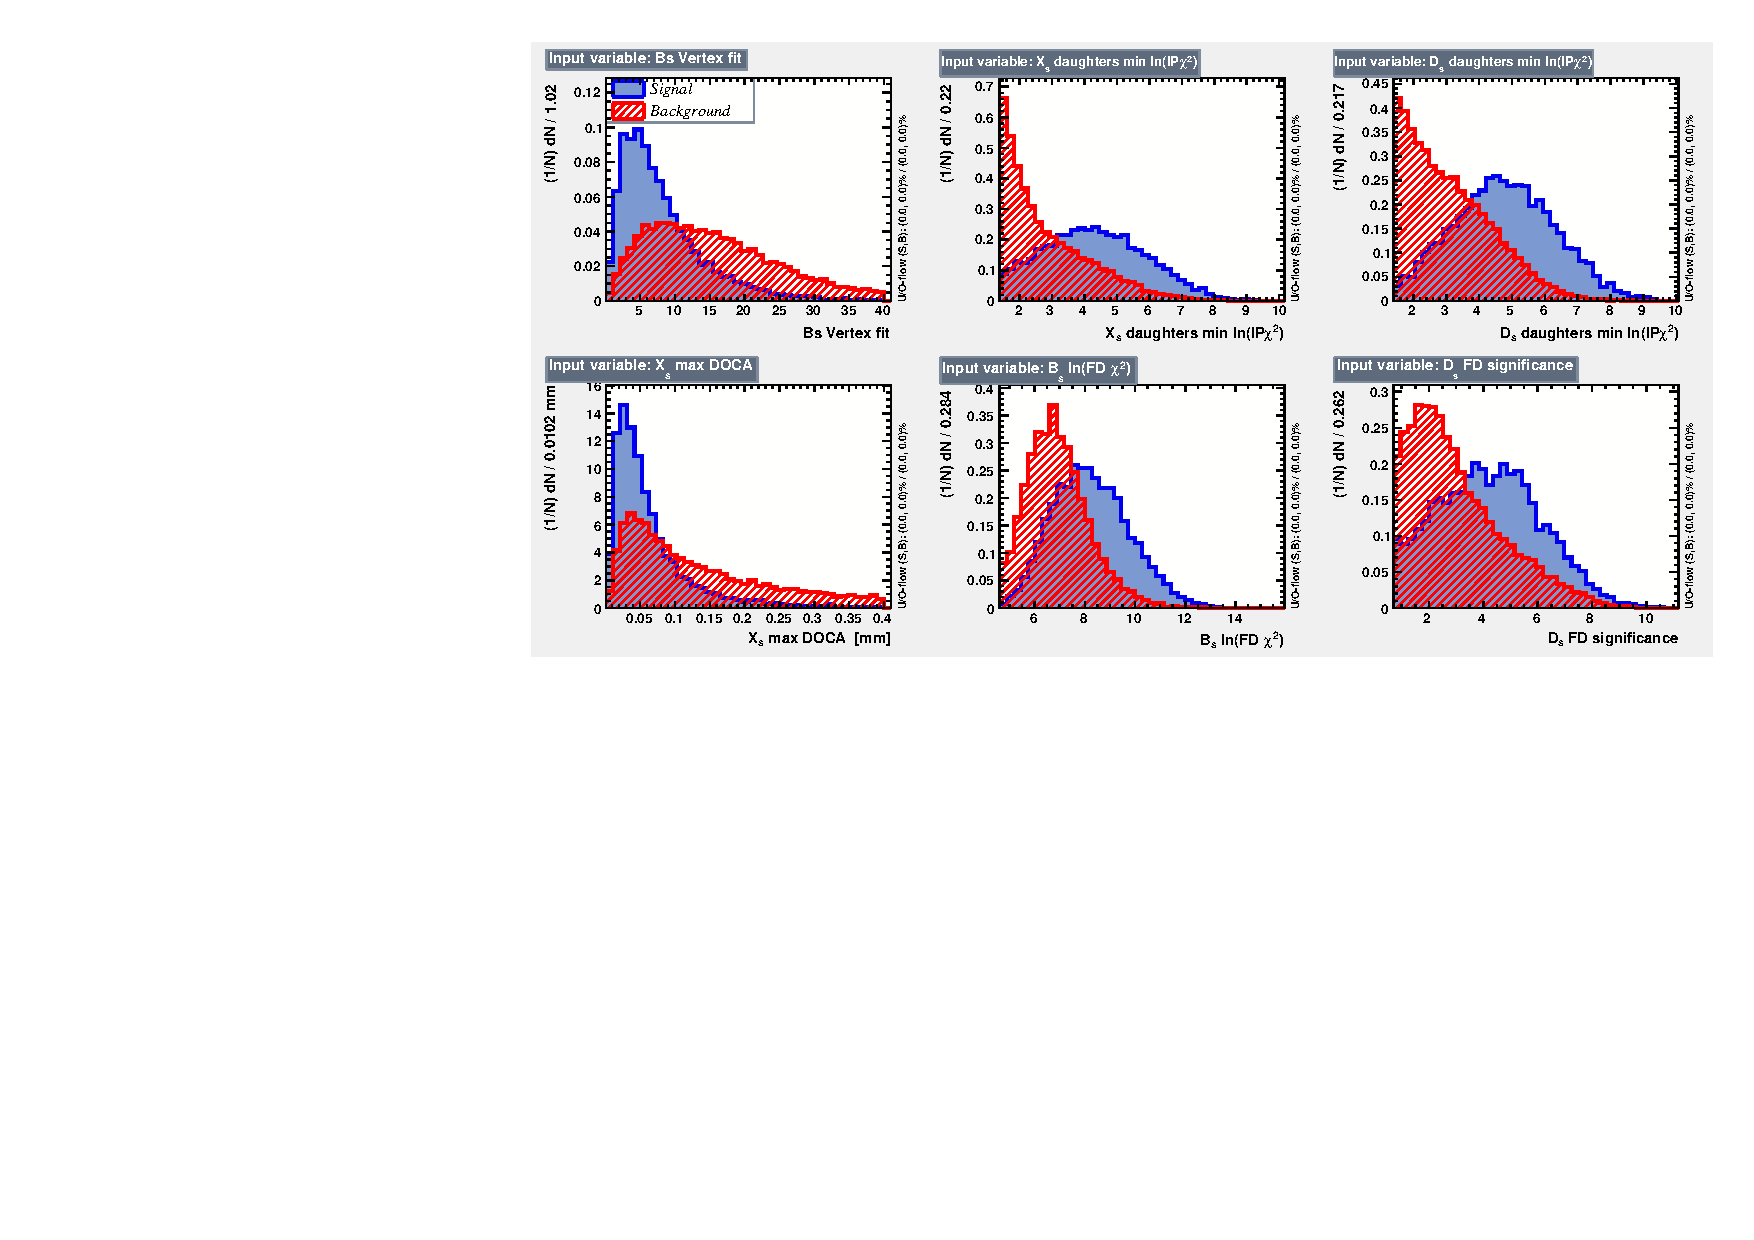
\includegraphics[height=6.cm,width=0.95\textwidth]{figs/BDT_Input_1.pdf}
%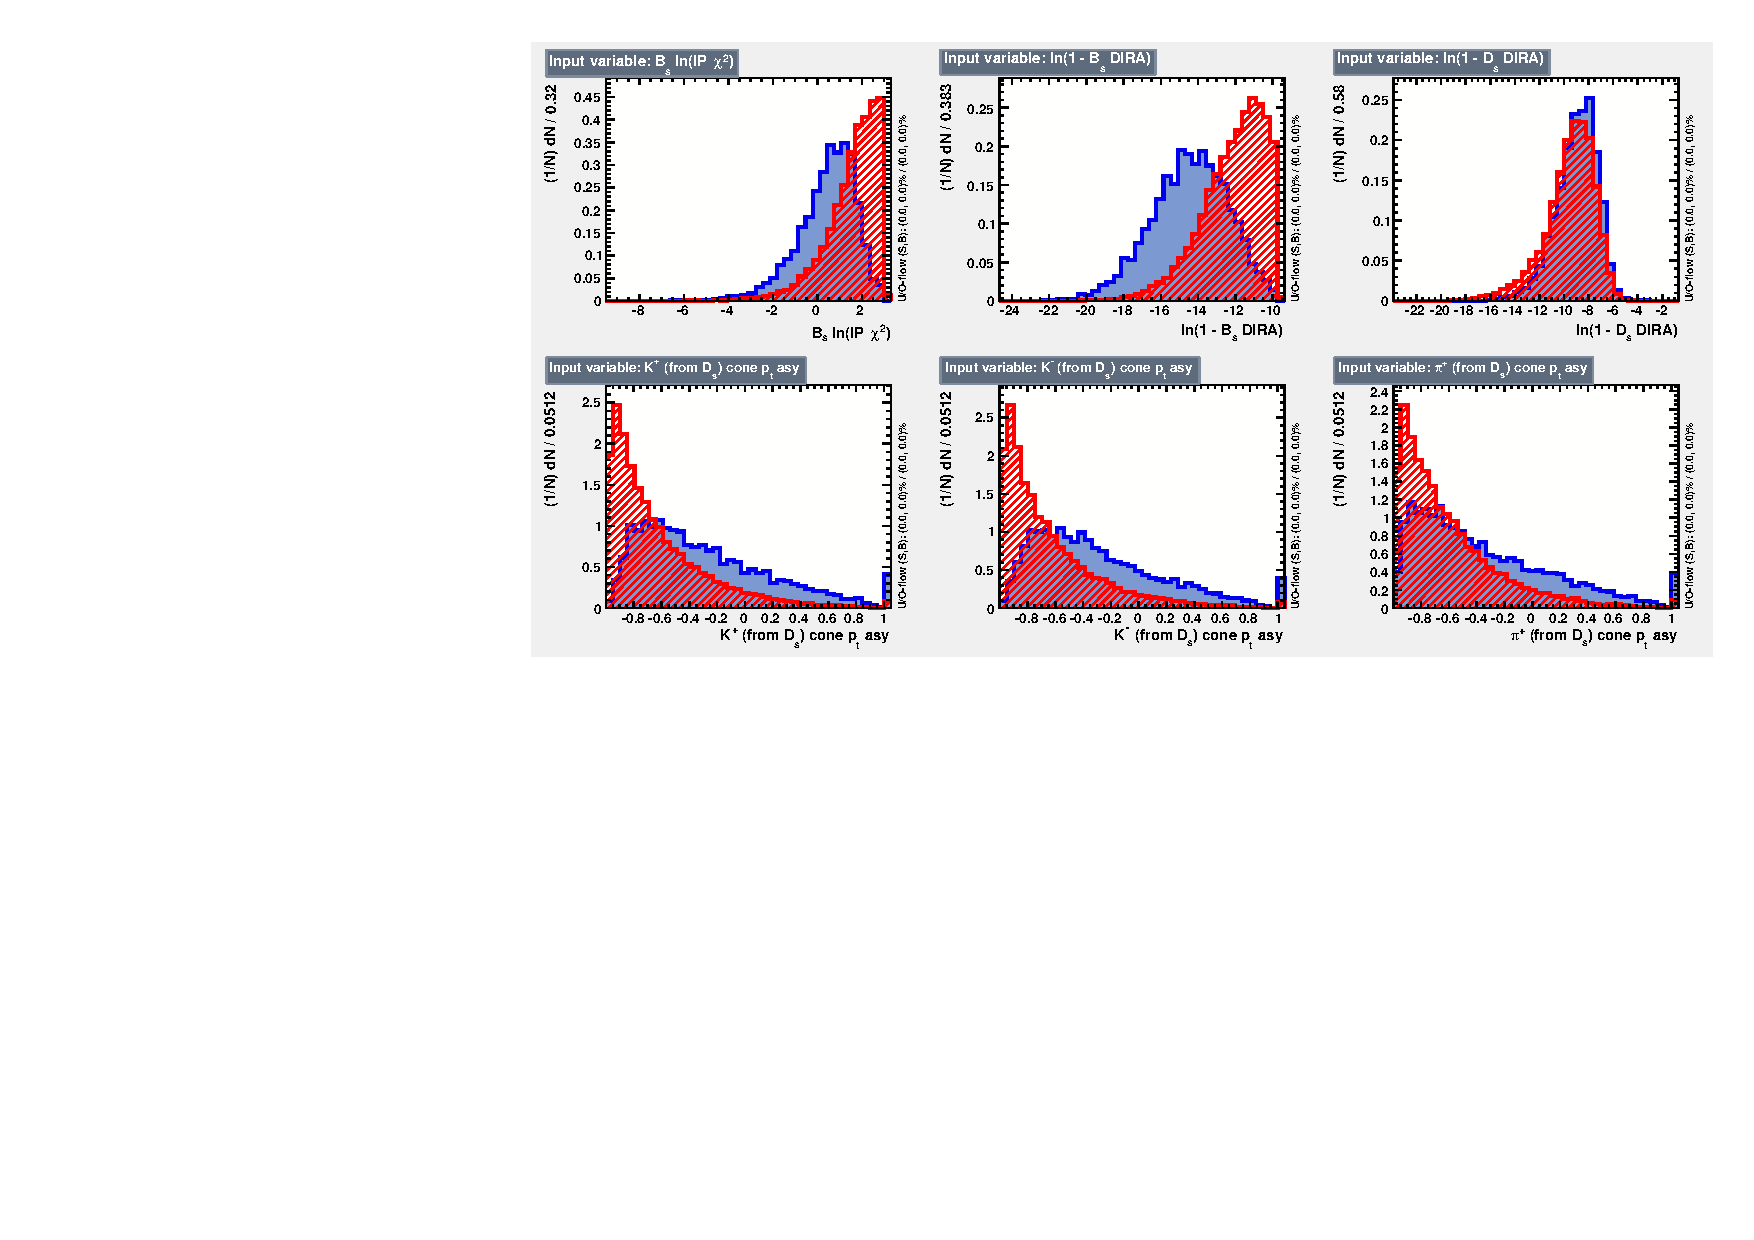
\includegraphics[height=6.cm,width=0.95\textwidth]{figs/BDT_Input_2.pdf}
%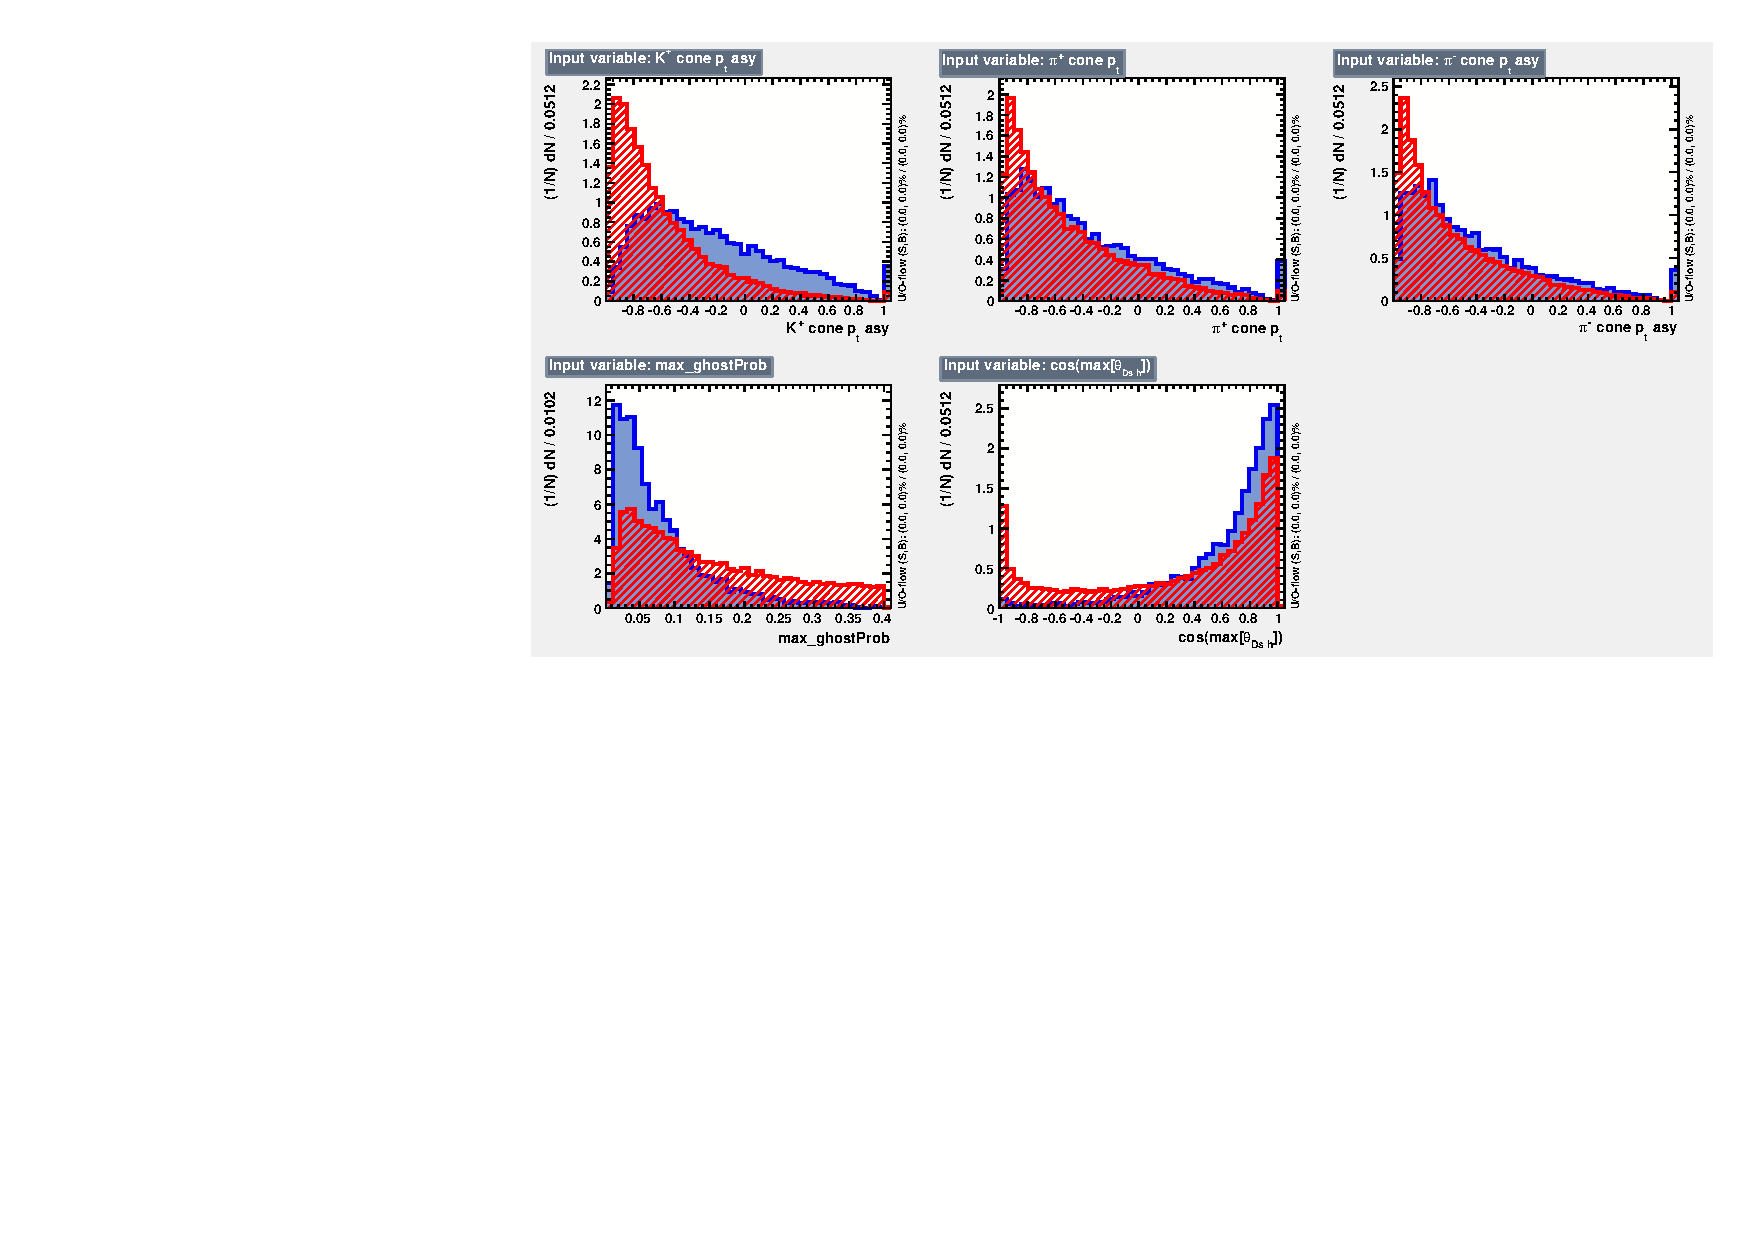
\includegraphics[height=6.cm,width=0.95\textwidth]{figs/BDT_Input_3.pdf}
%%\vspace*{-0.2cm}
%\caption{Distributions of the input variables used in the BDTG training. The background is shown as red hatched, while the signal is depicted solid blue.}
%\label{fig:BDT_Input_1}
%\end{figure}

%The relative importance of the input variables for the BDTG training is summarized in Table \ref{table:InputVars}.
%
%\begin{table}[h]
%\centering
% \begin{tabular}{l c}
%Variable & relative importance [$\%$]\\
%  \hline
%pi\_minus\_ptasy\_1.00 & 7.32\\
%log\_Ds\_FDCHI2\_ORIVX & 7.23\\
%K\_plus\_ptasy\_1.00 & 7.17\\
%log\_Ds\_DIRA & 6.96\\
%Bs\_ENDVERTEX\_CHI2 & 6.82\\
%max\_ghostProb & 6.76\\
%pi\_plus\_ptasy\_1.00 & 6.57\\
%log\_DsDaughters\_min\_IPCHI2 & 6.21\\
%log\_Bs\_DIRA & 6.15\\
%K\_plus\_fromDs\_ptasy\_1.00 & 6.10\\
%log\_XsDaughters\_min\_IPCHI2 & 5.87\\
%K\_minus\_fromDs\_ptasy\_1.00 & 5.62\\
%cos(Ds h) & 5.58\\
%log\_Bs\_IPCHI2\_OWNPV & 5.08\\
%log\_Bs\_FDCHI2\_OWNPV & 4.04\\
%Xs\_max\_DOCA & 3.98\\
%pi\_minus\_fromDs\_ptasy\_1.00 & 2.59\\
%\end{tabular}
%\caption{Summary of the relative importance of each variable in the training of the BDTG.}
%\label{table:InputVars}
%\end{table}

 
%\begin{figure}[h]
%%\vspace*{-0.4cm}
%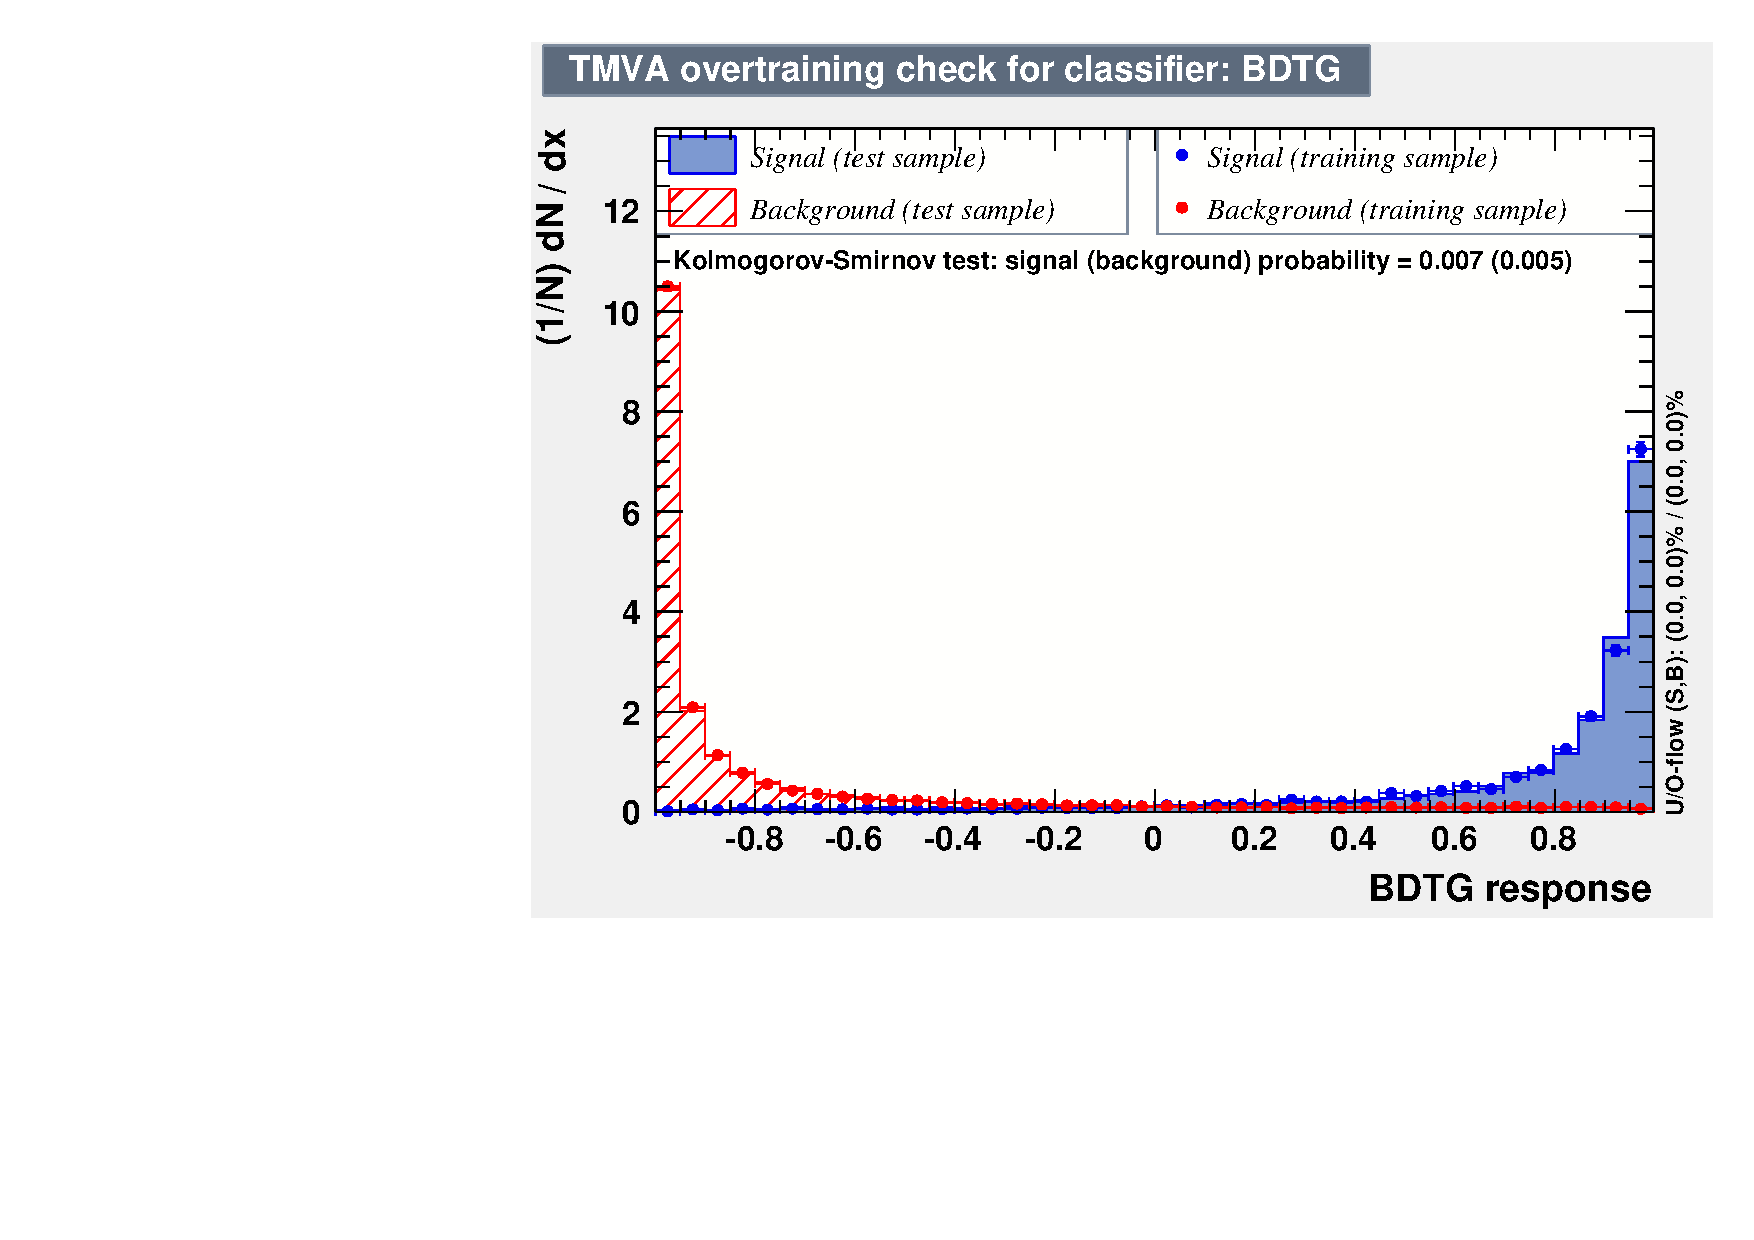
\includegraphics[height=7.4cm,width=0.7\textwidth]{figs/BDT_Response_new.pdf}
%%\vspace*{-0.2cm}
%\caption{BDTG output classifier distribution for (blue) signal and (red) background. The response of an independent test sample (dots) is overlaid.}
%\label{fig:BDT_Response}
%\end{figure}

       
%We determine the optimal cut value by maximizing the figure of merit $S/\sqrt{S+B}$ where S is the signal yield and B the background yield in the signal region, defined to be within $\pm$50 $\mevcc$ of the nominal $\Bs$ mass. 
%To avoid a bias in the determination of the branching fraction, we determine S and B using our normalization channel. 
%All trigger, stripping and additional selection criteria described in this and the previous chapter are applied to the $\Bs\to\Ds\pion\pion\pion$ data samples. 
%After that, we perform a simplified version of the fit to the invariant mass distribution of $\Bs\to\Ds\pion\pion\pion$ candidates described in Sec.~\ref{sec: fitting}.
%Here, a Gaussian function to model the signal and an exponential function to model combinatorial background is used.
%From this fit we estimate the number of signal events in our normalization channel. 
%Multiplying that number with the PDG branching fraction of $\frac{\mathcal{B}(\Bs\to\Ds\kaon\pion\pion)}{\mathcal{B}(\Bs\to\Ds\pion\pion\pion)}$ and the ratio of efficiencies discussed in Sec. \ref{sec: efficiency} allows us to estimate the expected number of $\Bs\to\Ds\kaon\pion\pion$ signal decays. The number of background events can then be computed as
%
%\begin{equation}
% N_{bkg}=N_{all}-N_{sig}|_{m_{\Bs\pm50\mevcc}}.   
%\end{equation}
%
%The efficiency curves as a function of the cut value are shown in Fig. \ref{fig:BDT_Efficiency}. 
%The optimal cut value is found to be BDTG $>$ 0.7012. At this working point the signal efficiency is estimated to be 72.47 $\%$, while the background rejection in the signal region is 97.38 $\%$. 


%\begin{figure}[h]
%%\vspace*{-0.4cm}
%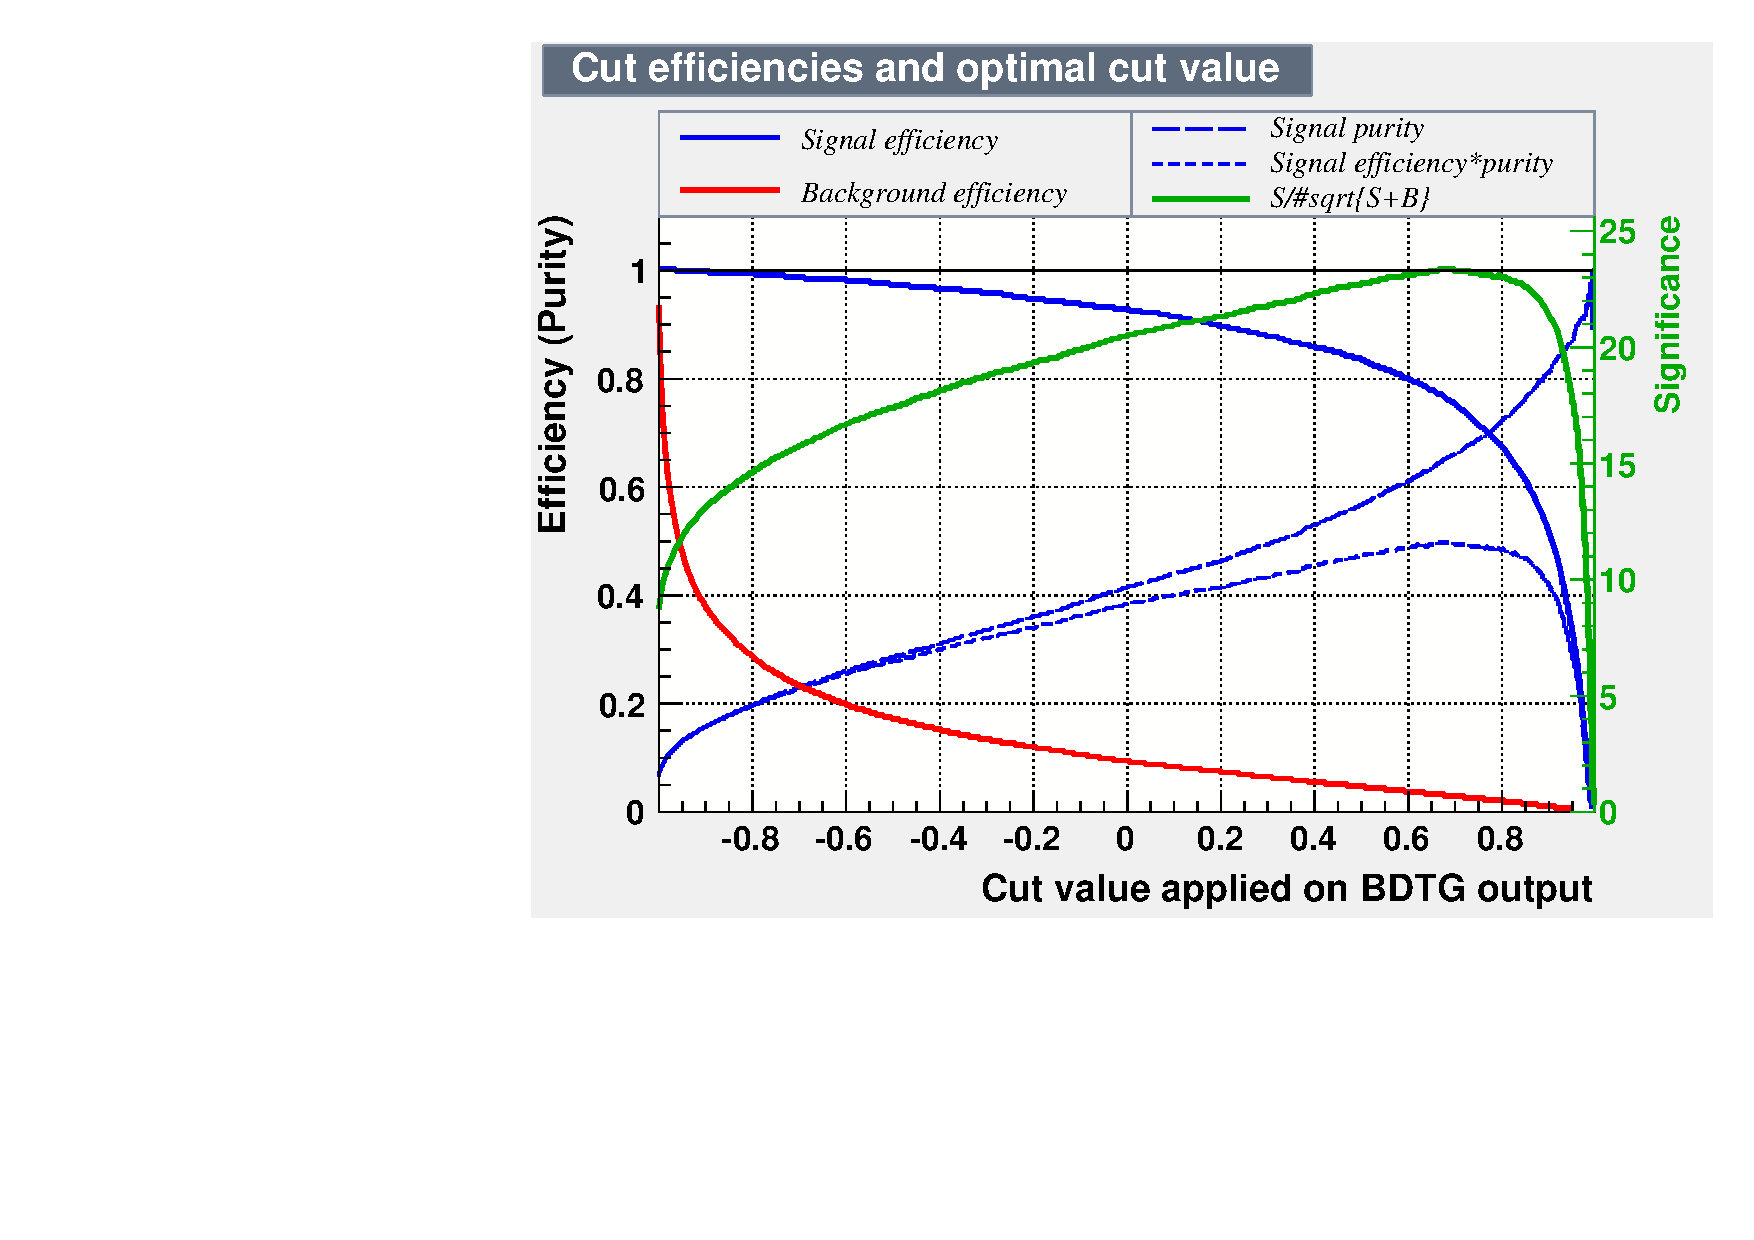
\includegraphics[height=7.4cm,width=0.7\textwidth]{figs/BDT_CutEfficiency.pdf}
%%\vspace*{-0.2cm}
%\caption{Efficiency and purity curves for (blue) signal, (red) background and the (green) FoM curve, as a function of the chosen cut value.}
%\label{fig:BDT_Efficiency}
%\end{figure}


\clearpage



\begin{table}[h]
\centering
\caption{Offline selection requirements for $D_s \to 3 h$ candidates.}
\resizebox{\linewidth}{!}{
 \renewcommand{\arraystretch}{1.}
 \small
 \begin{tabular}{l l l}
\hline
\hline
 & Description & Requirement  \\
\hline
$D_s \to h h h$ &  $m(hhh)$ & = $m_{D_s} \pm 20 \mev$  \\
\\
$D_s^- \to K K \pi^-$  & $D^0$ veto  & $m(K K) < 1840$ MeV \\
\\
$D_s^- \to \phi \pi^-$ & $m(KK)$  & $= m_{\phi} \pm 20$ MeV \\
& PIDK($K^+$) & $> -10$ \\
& PIDK($K^-$) & $> -10$ \\
& PIDK($\pi^-$) & $< 20$ \\
&  $\chi^{2}_{FD}$ & $> 0$ \\
&  FD in $z$  &$ > -1$ \\
& $D^-$ veto  & $m(\Kp K^-_\pi \pim) \ne m(D^-) \pm 30$ MeV  $||$ $\text{PIDK}(K^-) > 0$\\
& $\Lambda_c$ veto  & $m(\Kp K^-_p \pim) \ne m(\Lambda_c) \pm 30$ MeV   $||$ $\text{PIDK}(K^-)-\text{PIDp}(K^-) > 0$ \\
\\
$D_s^- \to K^{*}(892) K^-$ & $m(KK)$  & $\ne m_{\phi} \pm 20$ MeV \\
& $m(K^+\pi^-)$  & $= m_{K^{*}(892)} \pm 75$ MeV \\
& PIDK($K^+$) & $> -10$ \\
& PIDK($K^-$) & $> -5$ \\
& PIDK($\pi^-$) & $< 10$ \\
&  $\chi^{2}_{FD}$ & $> 2$ \\
&  FD in $z$  &$ > 0$ \\
& $D^-$ veto  & $m(\Kp K^-_\pi \pim) \ne m(D^-) \pm 30$ MeV  $||$ $\text{PIDK}(K^-) > 5$\\
& $\Lambda_c$ veto  & $m(\Kp K^-_p \pim) \ne m(\Lambda_c) \pm 30$ MeV   $||$ $\text{PIDK}(K^-)-\text{PIDp}(K^-) > 5$ \\
\\
$D_s^- \to (K K \pi^-)_{NR}$ & $m(KK)$  & $\ne m_{\phi} \pm 20$ MeV \\
& $m(K^+\pi^-)$  & $\ne m_{K^{*}(892)} \pm 75$ MeV \\
& PIDK($K^+$) & $> 5$ \\
& PIDK($K^-$) & $> 5$ \\
& PIDK($\pi^-$) & $< 10$ \\
&  $\chi^{2}_{FD}$ & $> 5$ \\
&  FD in $z$  &$ > 0$ \\
& $D^-$ veto  & $m(\Kp K^-_\pi \pim) \ne m(D^-) \pm 30$ MeV  $||$ $\text{PIDK}(K^-) > 20$\\
& $\Lambda_c$ veto  & $m(\Kp K^-_p \pim) \ne m(\Lambda_c) \pm 30$ MeV  $||$ $\text{PIDK}(K^-)-\text{PIDp}(K^-) > 5$ \\
\\
$D_s \to \pi \pi \pi$ & PIDK($\pi$) & $< 10$  \\
& PIDp($\pi$) & $< 10$ \\
& $D^0$ veto  & $m(\pip \pim) < 1700$ MeV \\
&  $\chi^{2}_{FD}$ & $> 9$ \\
&  FD in $z$  &$ > 0$ \\
\\
$D_s^- \to K^- \pip \pim$ & PIDK($K$) & $> 10$  \\
& PIDK($\pi$) & $< 5$ \\
& PIDp($\pi$) & $< 10$ \\
& $D^0$ veto  & $m(K^- \pip) < 1750$ MeV \\
&  $\chi^{2}_{FD}$ & $> 9$ \\
&  FD in $z$  &$ > 0$ \\
\\
\hline
\hline
\end{tabular}
}
\label{table:selDs}
\end{table}


\begin{table}[h]
\centering
\caption{Offline selection requirements for $B_s\to D_s K \pi\pi (D_s \pi\pi\pi)$ candidates.}
%\resizebox{\linewidth}{!}{
 \renewcommand{\arraystretch}{1.}
 \small
 \begin{tabular}{l l l}
\hline
\hline
 & Description & Requirement  \\
\hline
$B_s \to D_s h \pi \pi$  & $m(D_s h \pi \pi)$ & $> 5200 \mev$ \\
&  $\chi^{2}_{vtx}/\text{ndof}  $&$ <  8$ \\
& DIRA &$ > 0.99994$ \\
& $\chi^{2}_{FD}$ & $> 100$ \\
& $\chi^{2}_{IP}$ & $< 20$ \\
&  $\chi^{2}_{DTF}/\text{ndof} $&$   <  15 $ \\
& $t$  & $ > 0.4 \ps$ \\
& $\delta t$  & $ < 0.15 \ps$ \\
& Phasespace region & $m(h\pi\pi) < 1.95 \gev$ \\ & & $m(h\pi) < 1.2 \gev$ \\ & & $m(\pi\pi) < 1.2 \gev$ \\
& Wrong PV veto & nPV = 1 $||$  $\text{min}(\Delta\chi^{2}_{IP}) > 20$ \\
\\
$X_s^+ \to K^+ \pi^+ \pi^-$  & PIDK(K) & $> 10$ \\
& PIDK($\pi^+$) & $< 10$ \\
& PIDK($\pi^-$) & $< 5$ \\
& Semi.-lep. veto & isMuon($K^+$) = 0 \\
\\
$X_s^+ \to \pi^+ \pi^+ \pi^-$  & PIDK($\pi^+$) & $< 5$ \\
& PIDK($\pi^-$) & $< 10$ \\
& Semi.-lep. veto & isMuon($\pip$) = 0 \\

\hline
\hline
\end{tabular}
%}
\label{table:selBs}
\end{table}


\subsection{Simulation}




